%==============================================================================
%  Projektarbeit – Just-in-Time-Privilege-Elevation
%
%  Kompilieren:  pdflatex Projektarbeit.tex  (zweimal, wegen Inhaltsverzeichnis)
%  Schrift:      Latin Modern, 11pt, 1,5-zeilig
%  Klasse:       KOMA-Script (scrartcl)
%
%  Anpassen: Titelblock unten (Autor, Matrikelnummer, Betreuer, Hochschule).
%==============================================================================
\documentclass[11pt,a4paper]{article}

% --- Kodierung & Sprache -----------------------------------------------------
\usepackage[T1]{fontenc}
\usepackage[utf8]{inputenc}
\usepackage[ngerman]{babel}

% --- Schrift & Mikrotypografie ----------------------------------------------
\usepackage{lmodern}
\usepackage{microtype}     % feiner Randausgleich, Zeichenskalierung

% --- Seitenlayout ------------------------------------------------------------
\usepackage[
  left=3cm, right=2.5cm, top=2.5cm, bottom=2.5cm,
]{geometry}
\usepackage{setspace}
\onehalfspacing            % 1,5-facher Zeilenabstand
\usepackage{parskip}       % Absatzabstand statt Erstzeilen-Einzug

% --- Kopf-/Fußzeile ----------------------------------------------------------
\usepackage{fancyhdr}
\pagestyle{fancy}
\fancyhf{}
\fancyhead[L]{\small Just-in-Time-Privilege-Elevation}
\fancyhead[R]{\small\thepage}
\renewcommand{\headrulewidth}{0.4pt}

% --- Tabellen, Grafiken, Beschriftungen -------------------------------------
\usepackage{booktabs}
\usepackage{graphicx}
\usepackage{float}
\usepackage{flafter}           % Floats erscheinen nie vor ihrer Referenz
\usepackage{caption}
\captionsetup{font=small,labelfont=bf}
\raggedbottom                  % kein gestreckter Leerraum am Seitenende

% --- Farben & Quelltext-Listings --------------------------------------------
\usepackage{xcolor}
\definecolor{codebg}{HTML}{F6F8FA}
\definecolor{codekw}{HTML}{0B5394}
\definecolor{codestr}{HTML}{8B0000}
\definecolor{codecmt}{HTML}{6A737D}
\usepackage{listings}

\lstdefinelanguage{Go}{
  morekeywords={break,case,chan,const,continue,default,defer,else,fallthrough,%
    for,func,go,goto,if,import,interface,map,package,range,return,select,%
    struct,switch,type,var,nil,true,false,error,string,int,uint,uint64,bool,byte},
  sensitive=true,
  morecomment=[l]{//},
  morecomment=[s]{/*}{*/},
  morestring=[b]",
  morestring=[b]`,
}

\lstset{
  language=Go,
  basicstyle=\ttfamily\small,
  backgroundcolor=\color{codebg},
  keywordstyle=\color{codekw}\bfseries,
  stringstyle=\color{codestr},
  commentstyle=\color{codecmt}\itshape,
  numbers=left,
  numberstyle=\tiny\color{codecmt},
  numbersep=8pt,
  frame=single,
  rulecolor=\color{gray!40},
  breaklines=true,
  showstringspaces=false,
  tabsize=2,
  columns=fullflexible,
  keepspaces=true,
  inputencoding=utf8,
  extendedchars=true,
  literate=%
    {ä}{{\"a}}1 {ö}{{\"o}}1 {ü}{{\"u}}1 {ß}{{\ss}}1%
    {Ä}{{\"A}}1 {Ö}{{\"O}}1 {Ü}{{\"U}}1,
}

% --- Hyperlinks (dezent, druckfreundlich) -----------------------------------
\usepackage[hidelinks]{hyperref}

%==============================================================================
\begin{document}

%------------------------------------------------------------------ Titelseite
\begin{titlepage}
  \centering
  {\scshape\large Methoden und Werkzeuge der Softwareentwicklung\par}
  \vspace{0.5cm}
  {\scshape Projektarbeit\par}
  \vfill
  {\Huge\bfseries Just-in-Time-Privilege-Elevation\par}
  \vspace{0.8cm}
  {\Large Ein Modul für zeitlich befristete,\\[0.2em]
   zwei-faktor-gesicherte Rechte-Erhöhung\par}
  \vfill
  \begin{tabular}{rl}
    Autor:        & Lukas Cvitanović \\        % <- anpassen
    Matrikelnr.:  & \rule{4cm}{0.4pt} \\        % <- anpassen
    Kurs:         & \rule{4cm}{0.4pt} \\        % <- anpassen
    Betreuer:     & \rule{4cm}{0.4pt} \\        % <- anpassen
  \end{tabular}
  \vspace{1.5cm}

  {\large \today\par}
\end{titlepage}

%--------------------------------------------------------- Inhaltsverzeichnis
\tableofcontents
\clearpage

%==============================================================================
\section{Einleitung und Motivation}

Administrative Berechtigungen werden in vielen Systemen dauerhaft vergeben:
Ein Konto besitzt erhöhte Rechte unabhängig davon, ob diese im Moment
tatsächlich benötigt werden. Diese Praxis widerspricht dem
Least-Privilege-Prinzip und vergrößert den potenziellen Schaden einer
Kontoübernahme erheblich, da ein kompromittiertes Administratorkonto jederzeit
voll handlungsfähig ist. Zugleich erschwert sie die Nachvollziehbarkeit: Aus
einer dauerhaften Rechtevergabe lässt sich nicht ablesen, wann und wozu ein
Recht tatsächlich ausgeübt wurde.

Als Antwort darauf hat sich \emph{Just-in-Time}-Zugriff (JIT) als Stand der
Technik etabliert. Erhöhte Rechte werden nur für den konkreten Bedarfsmoment
gewährt und laufen anschließend automatisch ab. Der Zeitraum, in dem ein
kompromittiertes Konto Schaden anrichten kann, wird damit auf wenige Minuten
begrenzt, und jede Erhöhung wird zu einem protokollierbaren Ereignis.

Die vorliegende Arbeit entwirft und implementiert ein eigenständiges,
wiederverwendbares Modul, das JIT-Privilege-Elevation als Bibliothek
bereitstellt. Das Modul ist bewusst vom Trägersystem entkoppelt und wird
beispielhaft in eine bestehende, selbst entwickelte PaaS-Umgebung integriert.
Nach der Anforderungsanalyse (Abschnitt~2) und der Einordnung in den Stand der
Technik (Abschnitt~3) beschreibt Abschnitt~4 das Konzept, Abschnitt~5 die
Sicherheitsanalyse nach STRIDE, Abschnitt~6 die Implementierung und
Abschnitt~7 die Evaluation.

%==============================================================================
\section{Anforderungen}

\subsection{Funktionale Anforderungen}
\begin{itemize}
  \item Ein Benutzer kann eine zeitlich befristete Rechte-Erhöhung
        \emph{beantragen}.
  \item Die Erhöhung wird erst nach erneuter Zwei-Faktor-Bestätigung
        (Step-Up-Authentication) wirksam.
  \item Aktive Erhöhungen lassen sich vorzeitig widerrufen und laufen
        andernfalls automatisch ab.
  \item Jeder Schritt wird manipulationssicher protokolliert.
\end{itemize}

\subsection{Nicht-funktionale Anforderungen}
\begin{description}
  \item[Fail-closed] Im Zweifel oder bei jedem Fehler wird kein Recht gewährt.
  \item[Unabhängigkeit] Der Kern ist vom Trägersystem entkoppelt
        (Ports-and-Adapters).
  \item[Nachvollziehbarkeit] Lückenloser, integritätsgesicherter Audit-Trail.
  \item[Korrektheit] Verifiziert durch automatisierte Tests inklusive
        Nebenläufigkeit.
\end{description}

%==============================================================================
\section{Stand der Technik}

Verfahren zur kontrollierten Rechteerhöhung sind etabliert; sie unterscheiden
sich vor allem in Granularität und Betriebsaufwand. \emph{HashiCorp Vault}
stellt über seine SSH-Secrets-Engine kurzlebige, signierte SSH-Zertifikate aus
und verlagert die Rechteerhöhung damit auf die Betriebssystemebene; dies setzt
allerdings eine eigene Public-Key-Infrastruktur voraus. \emph{HashiCorp
Boundary} und \emph{Teleport} schalten einen Sitzungs-Broker mit vollständiger
Sitzungsaufzeichnung vor -- sehr mächtig, aber mit erheblichem Betriebsaufwand
verbunden. Identity-Provider wie \emph{Keycloak} oder \emph{Authentik} bieten
Step-Up-Authentifizierung auf Basis von OpenID Connect, sind dabei jedoch auf
den jeweiligen Identity-Provider zentriert.

Tabelle~\ref{tab:sota} ordnet diese Systeme ein. Das in dieser Arbeit
entwickelte Modul verfolgt einen bewusst leichtgewichtigen Ansatz: Es führt die
Rechteerhöhung nicht als externe Infrastruktur, sondern als eingebettete
Bibliothek innerhalb der Anwendung durch. Dadurch entfällt zusätzlicher
Betriebsaufwand, und das Modul bleibt durch das Ports-and-Adapters-Muster
unabhängig vom konkreten Trägersystem.

\begin{table}[htbp]
  \centering
  \caption{Einordnung verwandter Systeme}
  \label{tab:sota}
  \begin{tabular}{@{}lll@{}}
    \toprule
    \textbf{System} & \textbf{Ansatz} & \textbf{Abgrenzung} \\
    \midrule
    HashiCorp Vault (SSH)      & kurzlebige SSH-Zertifikate     & OS-Ebene, eigene Infrastruktur \\
    Boundary / Teleport        & Session-Broker mit Recording   & mächtig, hoher Betriebsaufwand \\
    Keycloak / Authentik       & OIDC-basierte Re-Auth          & Identity-Provider-zentriert \\
    \textbf{Dieses Modul}      & eingebettete JIT-Erhöhung      & leichtgewichtig, integrierbar \\
    \bottomrule
  \end{tabular}
\end{table}

%==============================================================================
\section{Konzept und Architektur}

\subsection{Überblick}
Das Modul folgt dem Ports-and-Adapters-Muster: Der Kern kennt das Host-System
nicht, sondern spricht ausschließlich gegen Interfaces. Der Host stellt
konkrete Implementierungen bereit (Abbildung~\ref{fig:arch}).

\begin{figure}[htbp]
  \centering
  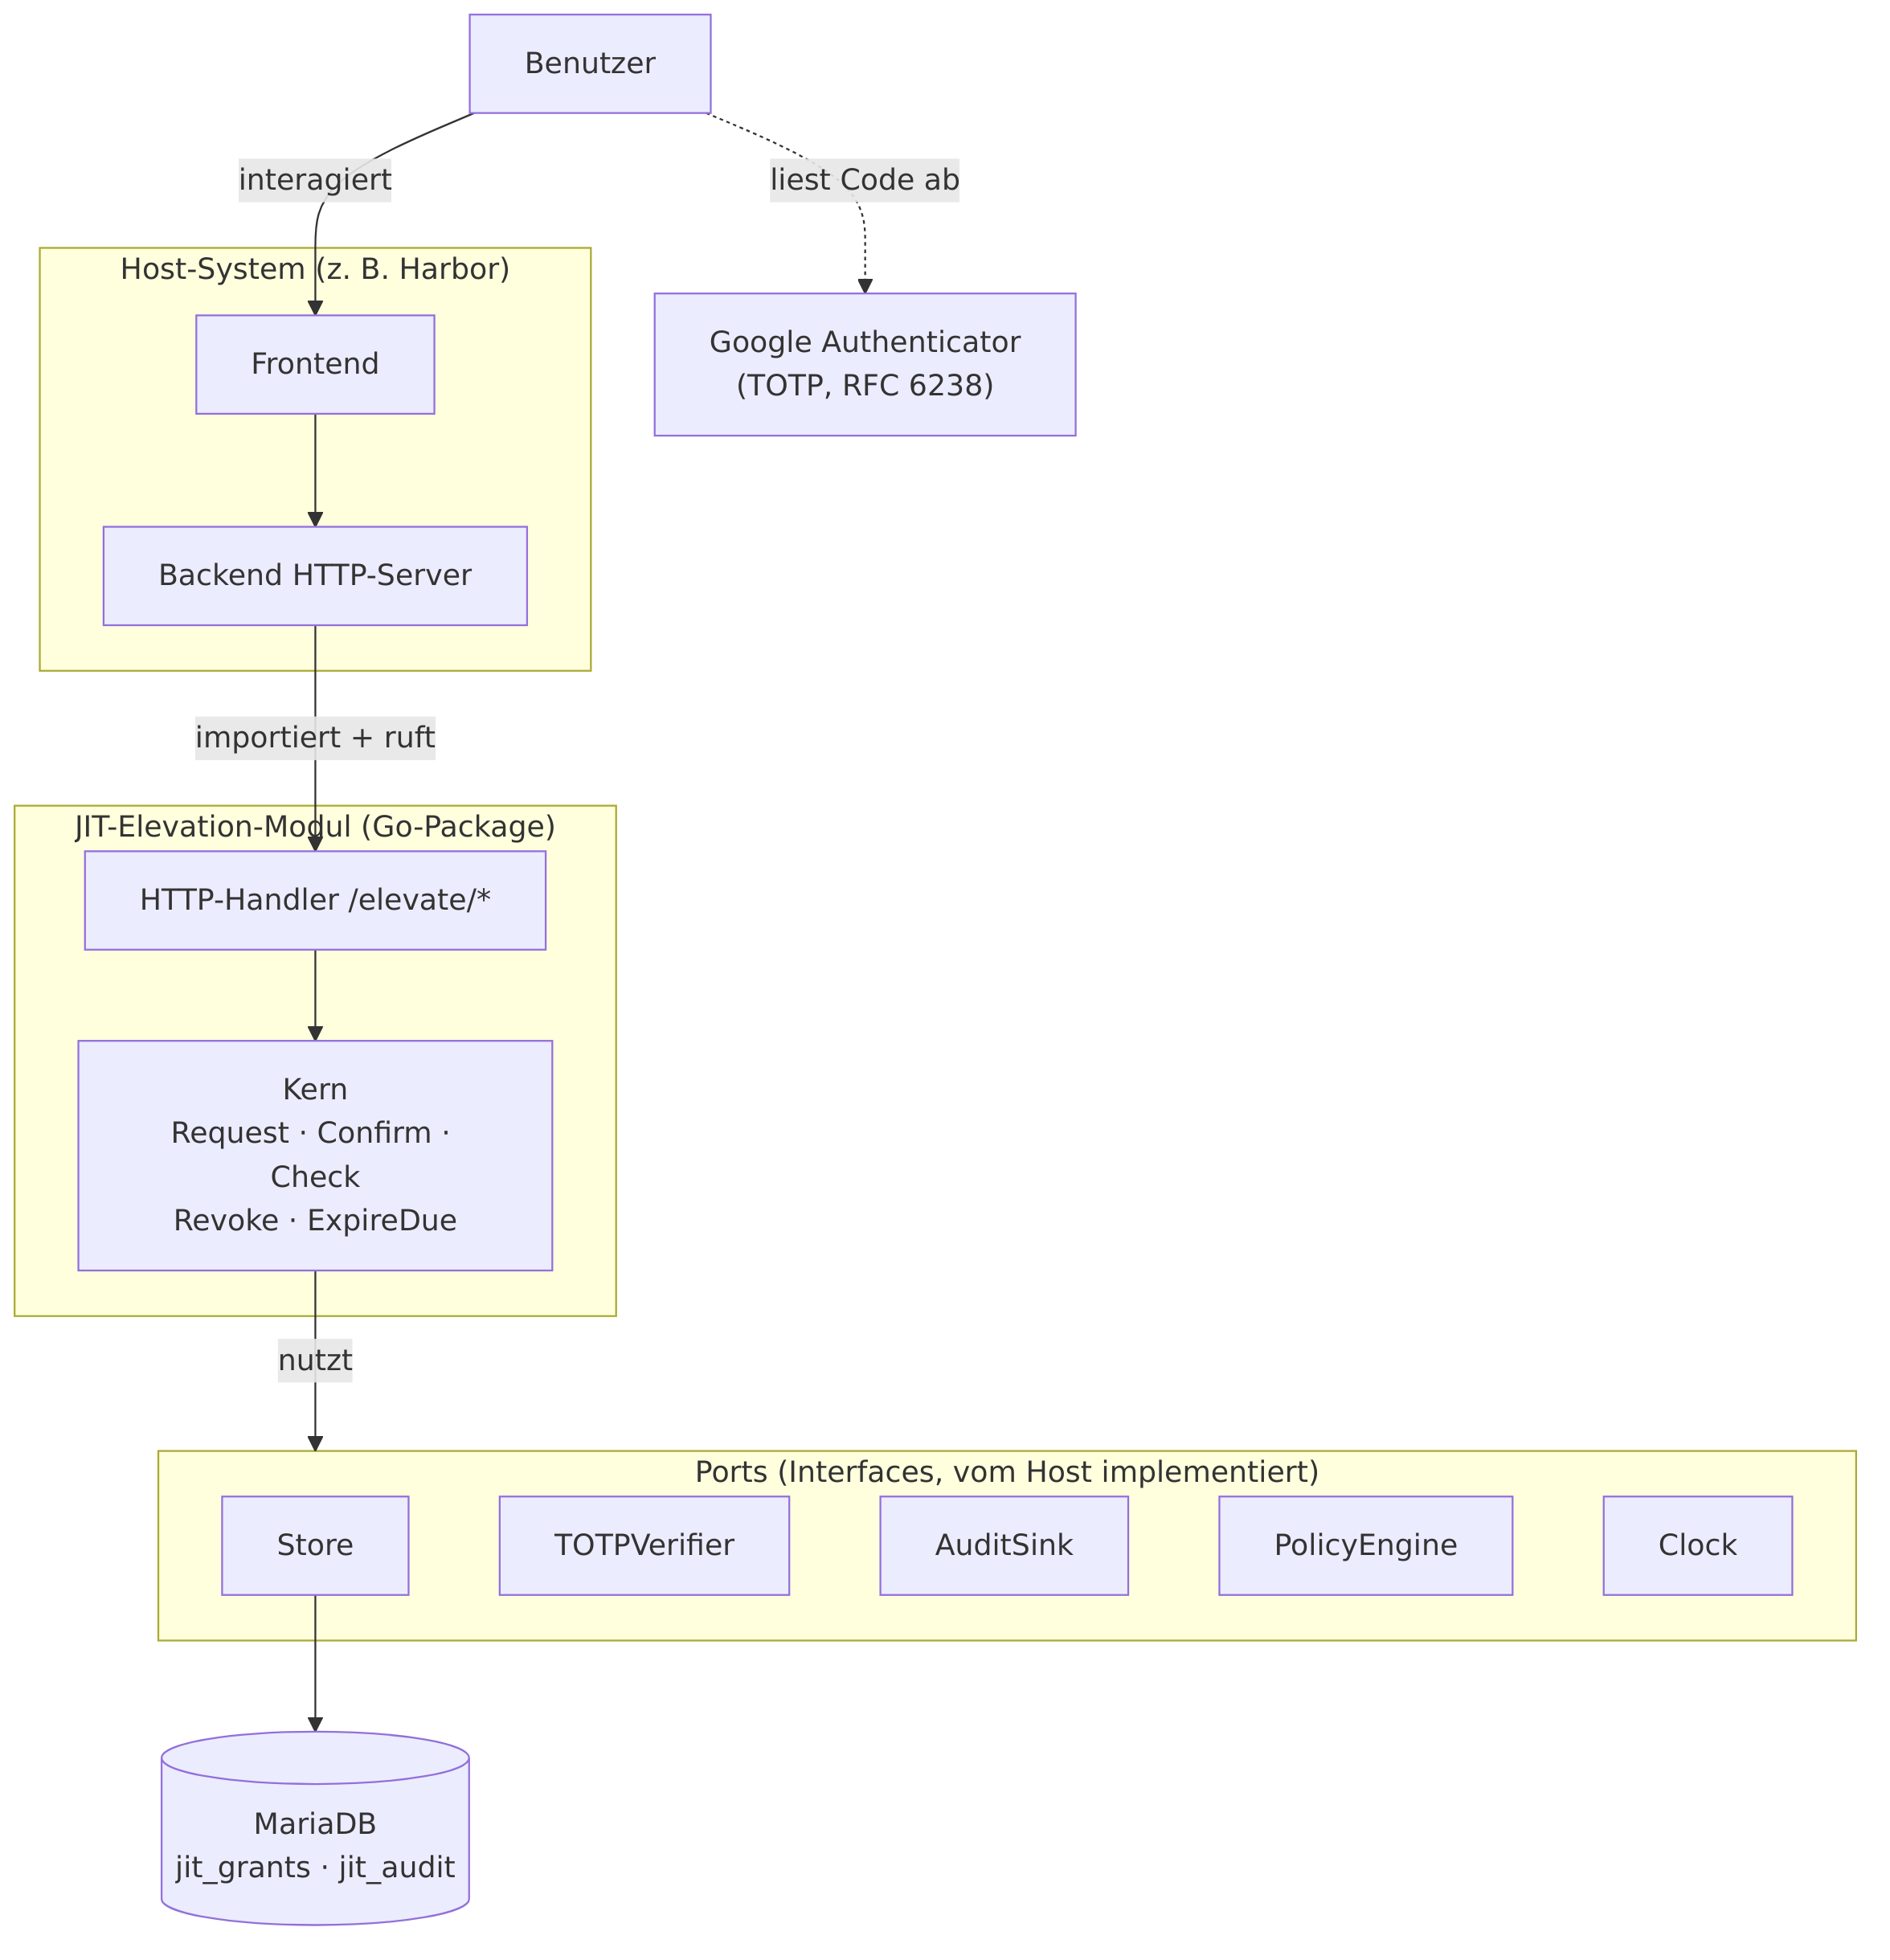
\includegraphics[width=\textwidth]{figures/diagram1.png}
  \caption{Architektur: Kern, Host und Adapter-Interfaces}
  \label{fig:arch}
\end{figure}

\subsection{Lebenszyklus eines Grants}
Eine Rechte-Erhöhung (Grant) durchläuft eine Zustandsmaschine
(Abbildung~\ref{fig:state}). Alle Endzustände sind terminal -- ein
abgelaufener, widerrufener oder abgelehnter Grant wird nie wieder aktiv
(fail-closed).

\begin{figure}[htbp]
  \centering
  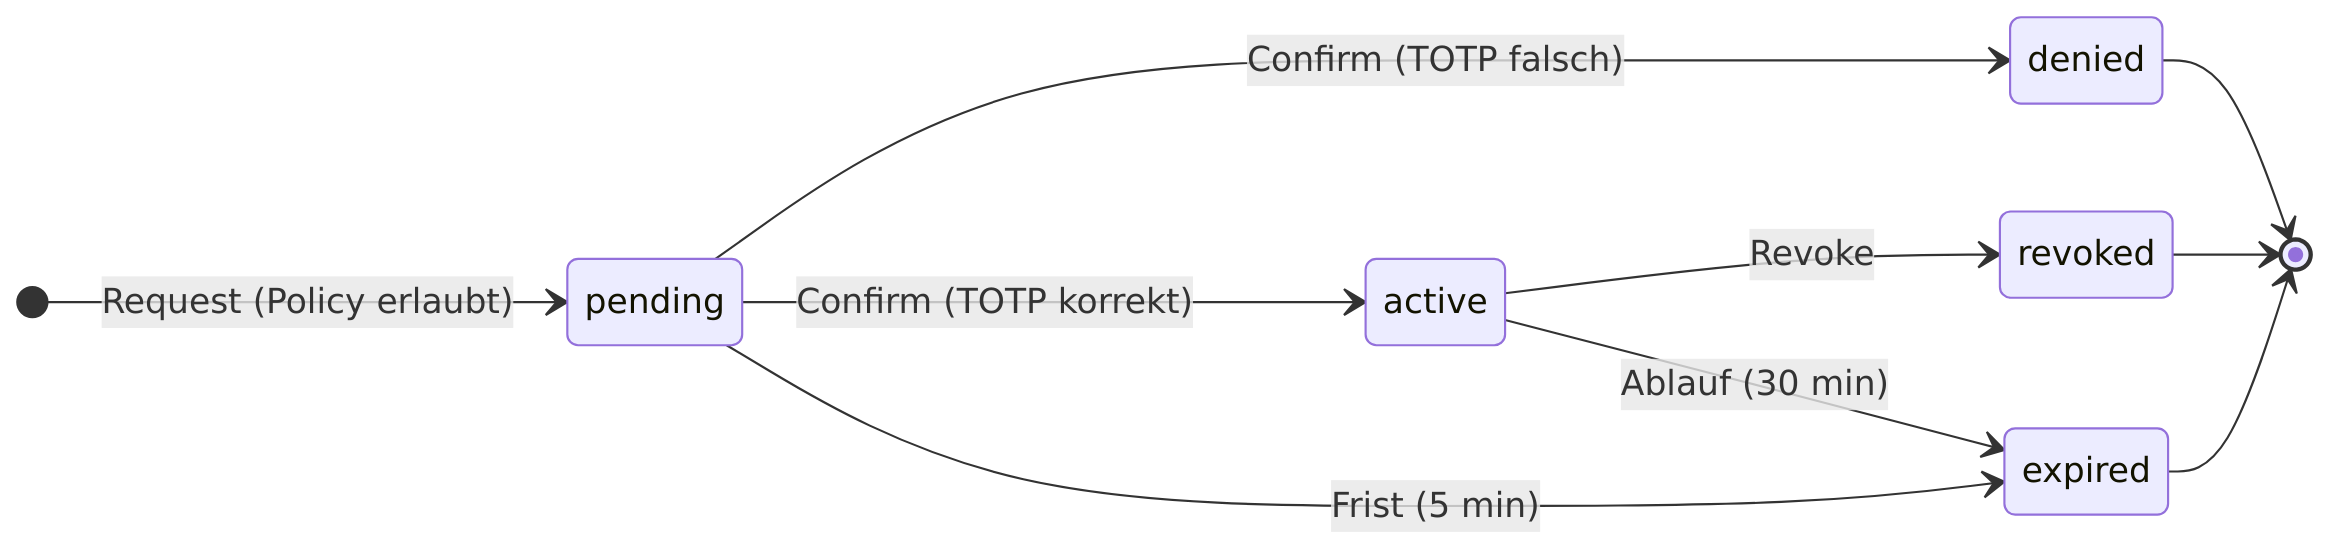
\includegraphics[width=0.95\textwidth]{figures/diagram2.png}
  \caption{Zustandsmaschine eines Grants}
  \label{fig:state}
\end{figure}

\subsection{Ablauf}
Der vollständige Ablauf umfasst vier Phasen (Abbildung~\ref{fig:seq}). Phase~2
ist der Step-Up-Moment: ohne gültigen zweiten Faktor entsteht keine aktive
Erhöhung.

\begin{figure}[htbp]
  \centering
  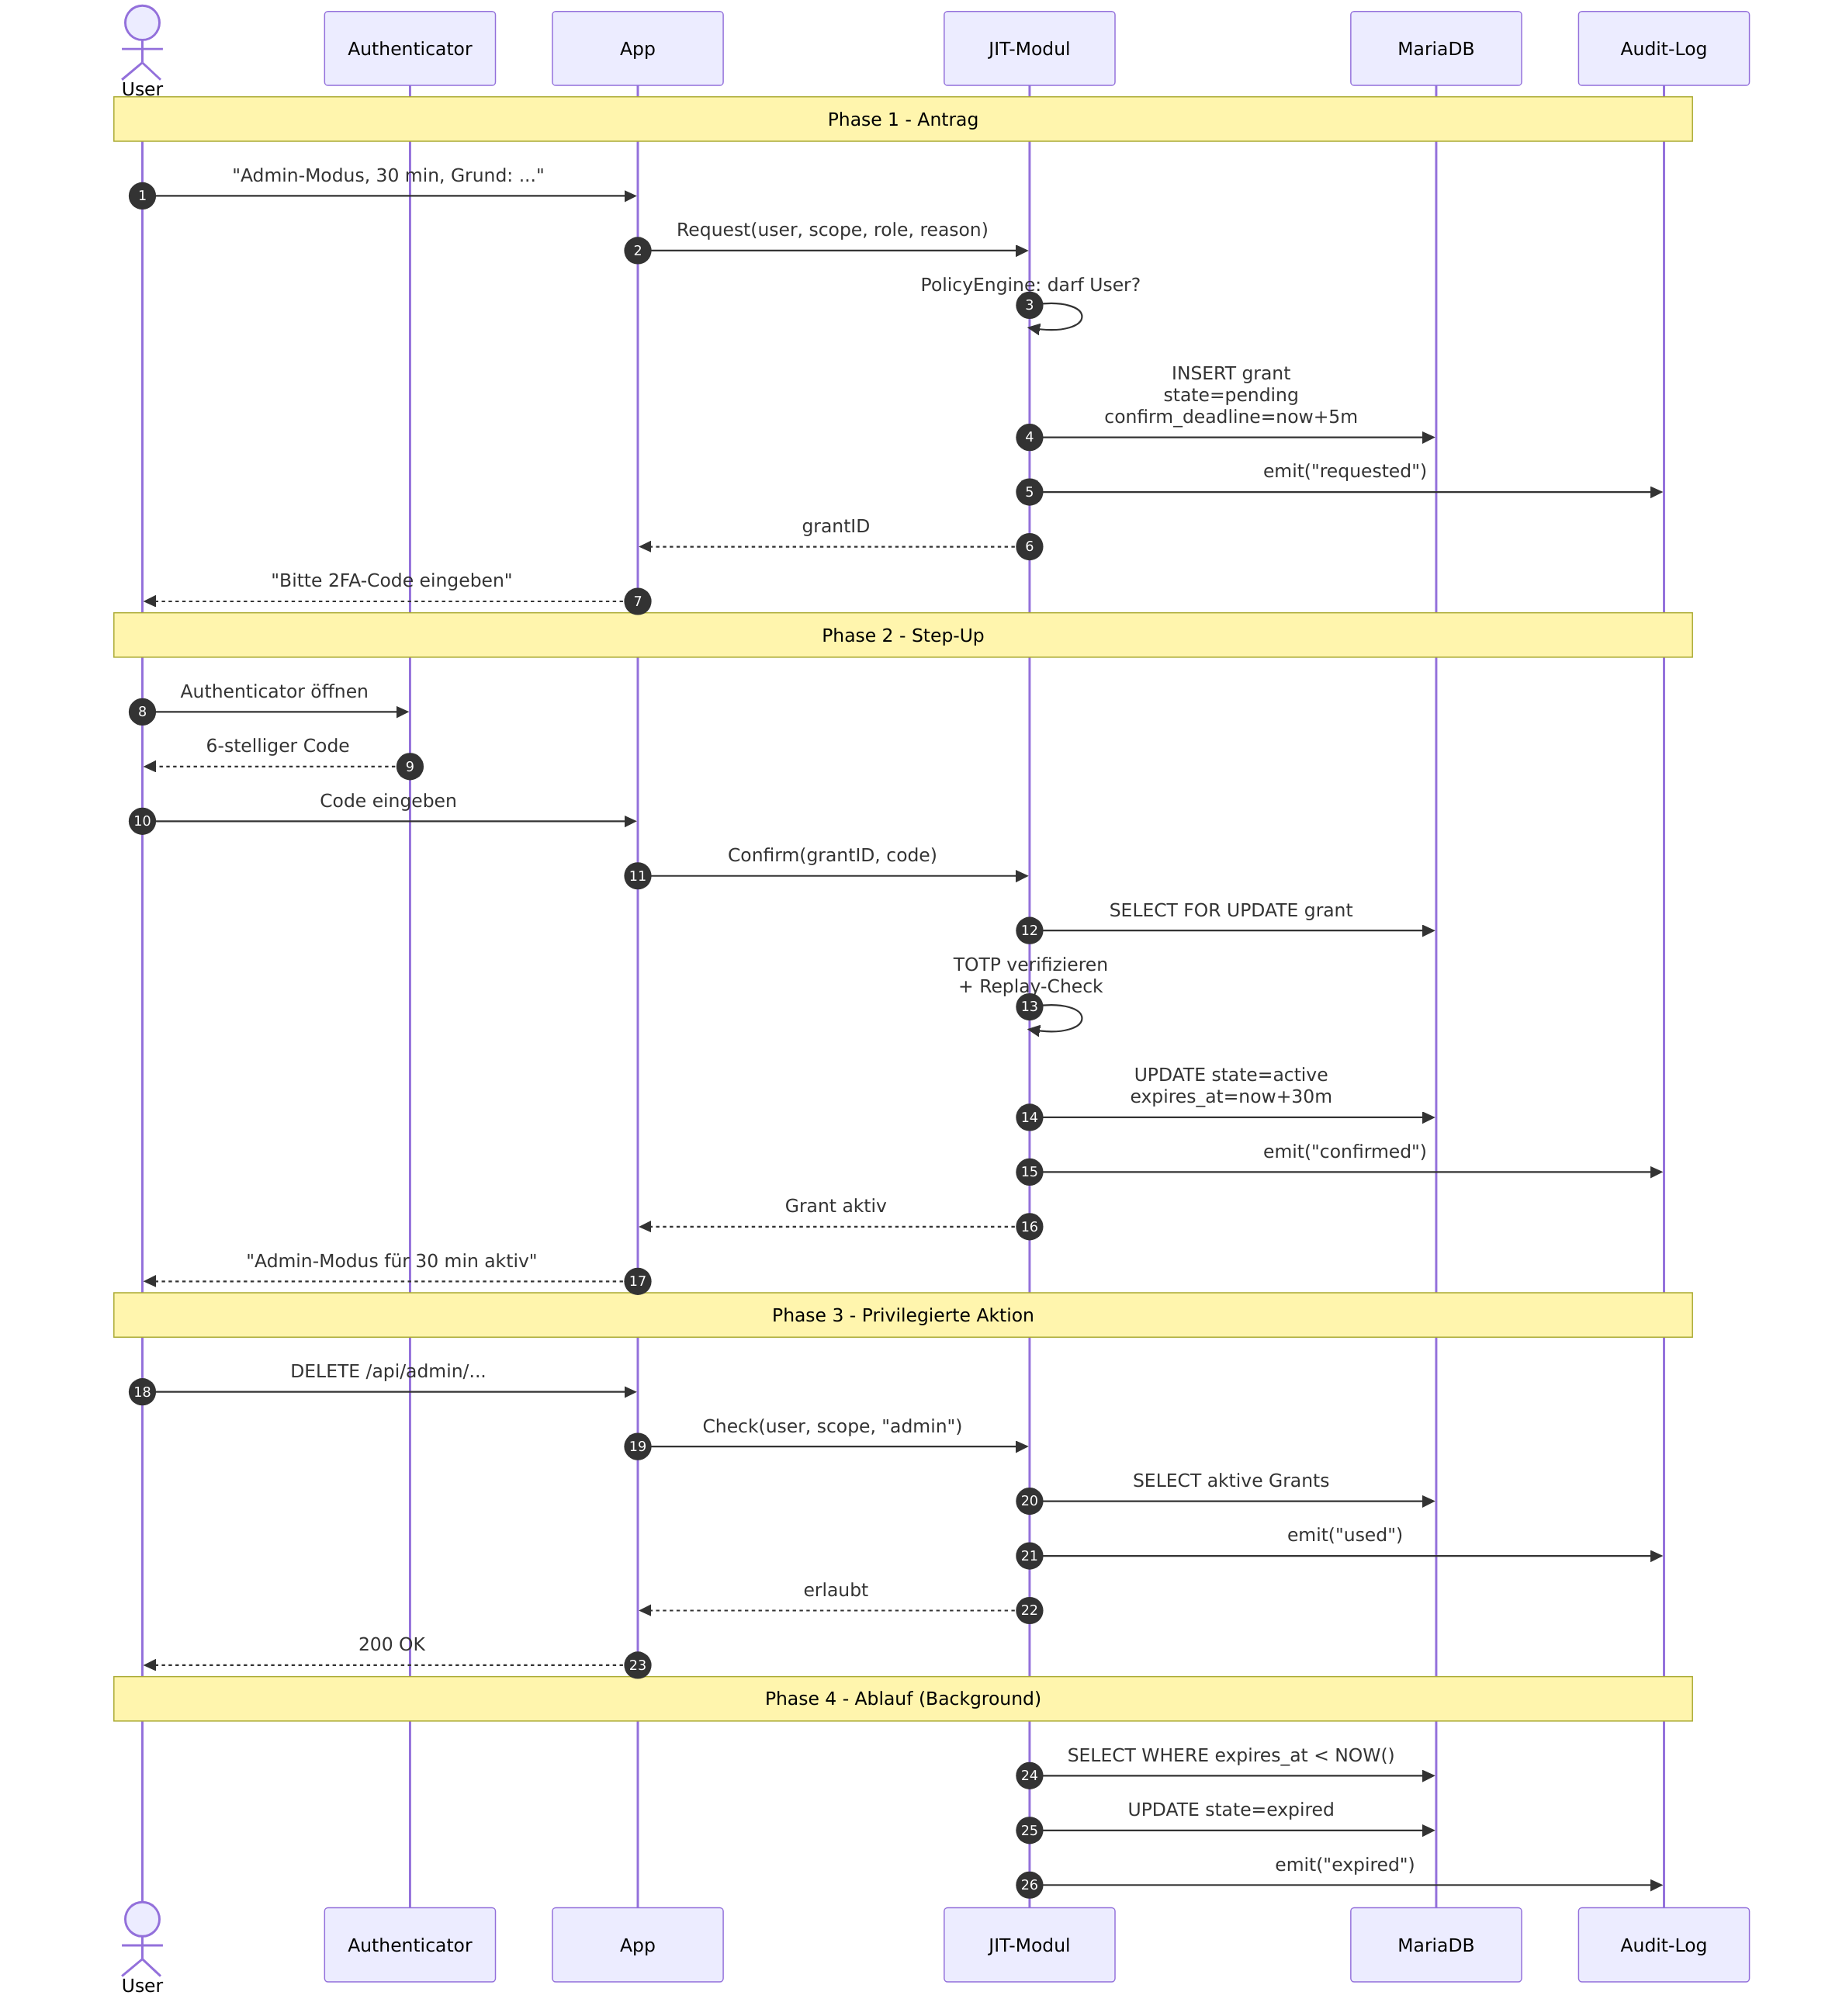
\includegraphics[width=\textwidth,height=0.88\textheight,keepaspectratio]{figures/diagram3.png}
  \caption{Ablauf: Antrag, Bestätigung, Nutzung, Ablauf}
  \label{fig:seq}
\end{figure}

\subsection{Datenmodell}
Das Modul legt drei Tabellen an (Abbildung~\ref{fig:er}): die Grants selbst,
das Audit-Log sowie eine Tabelle der bereits verbrauchten TOTP-Zeitfenster für
den benutzerweiten Replay-Schutz. Die Audit-Tabelle bildet eine Hash-Kette:
jede nachträgliche Manipulation eines Eintrags bricht die Kette am
Folgeeintrag.

\begin{figure}[htbp]
  \centering
  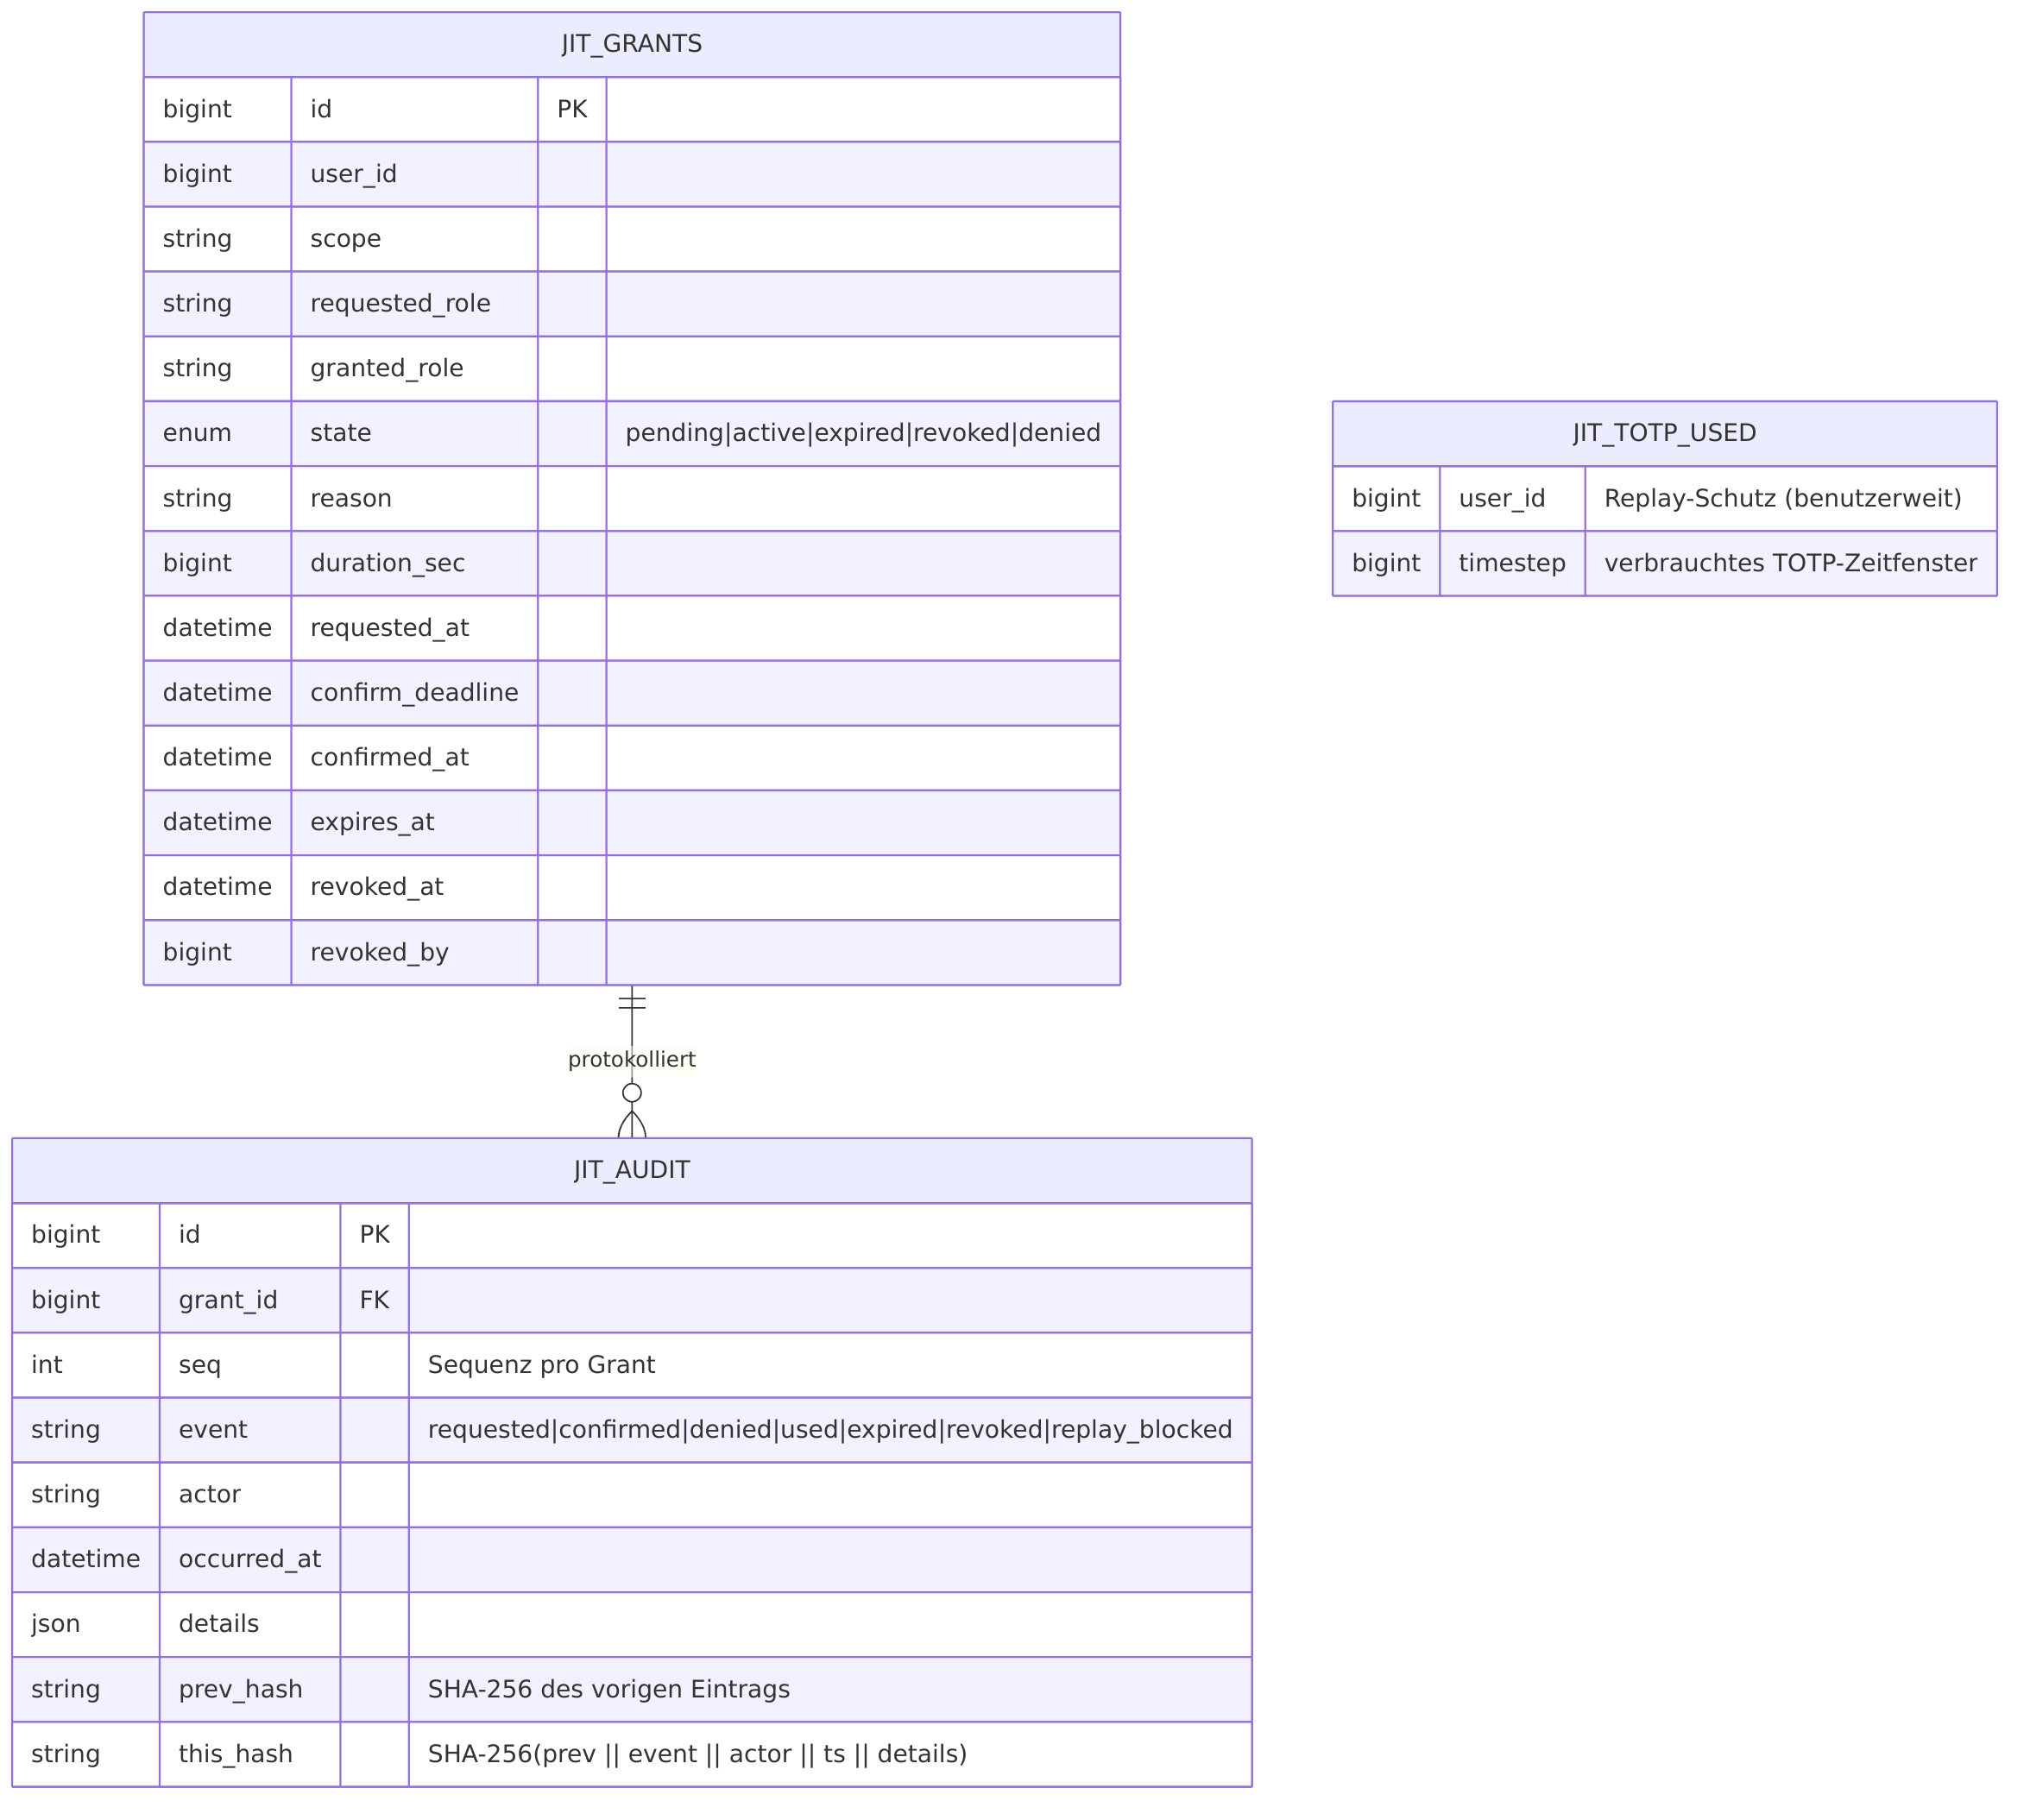
\includegraphics[width=\textwidth]{figures/diagram4.png}
  \caption{Datenmodell mit Audit-Hash-Kette}
  \label{fig:er}
\end{figure}

%==============================================================================
\section{Sicherheitsanalyse}

\subsection{Vertrauensgrenzen}
\begin{figure}[htbp]
  \centering
  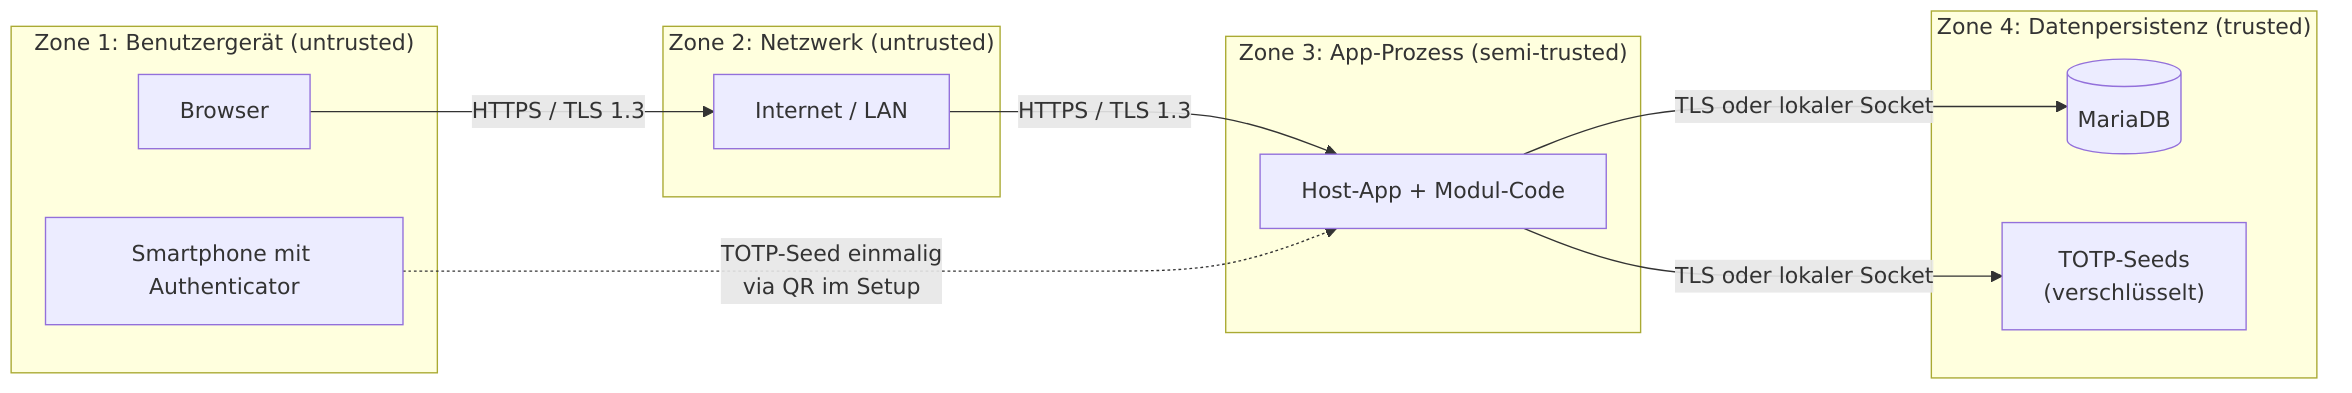
\includegraphics[width=\textwidth]{figures/diagram5.png}
  \caption{Vertrauensgrenzen als Grundlage der STRIDE-Analyse}
  \label{fig:trust}
\end{figure}

Drei Grenzen müssen kryptografisch geschützt sein: Browser $\leftrightarrow$
Backend (TLS), Backend $\leftrightarrow$ Datenbank (TLS oder lokaler Socket)
und der TOTP-Seed, der die Persistenz nie im Klartext verlässt.

\subsection{Bedrohungsanalyse nach STRIDE}
Die Analyse ordnet jeder Bedrohung eine konkrete Gegenmaßnahme im Entwurf bzw.
im Code zu. Annahmen: Der Host authentifiziert die Primäridentität; TLS sichert
den Transport; der TOTP-Seed liegt verschlüsselt im Secret-Store.

\paragraph{S -- Spoofing.} Erhöhung nur nach gültigem TOTP, den nur der echte
Benutzer besitzt (Step-Up, \texttt{Confirm} Schritt~1). Restrisiko:
kompromittierte Session \emph{und} Seed -- Minderung durch WebAuthn (Future
Work).

\paragraph{T -- Tampering.} Audit-Manipulation wird durch die SHA-256-Hash-Kette
erkennbar (\texttt{audit.go}); Grant-Daten sind nur über atomare Store-Methoden
änderbar; TLS schützt Daten im Transit.

\paragraph{R -- Repudiation.} Lückenloses Protokoll aller Ereignisse
(\texttt{requested}, \texttt{confirmed}, \texttt{used}, \texttt{revoked},
\texttt{expired}, \texttt{denied}, \texttt{replay\_blocked}); auf kritischen
Pfaden ist das Audit Pflicht -- keine Erhöhung ohne Spur.

\paragraph{I -- Information Disclosure.} TOTP-Seeds werden vom Persistenz-Adapter
verschlüsselt abgelegt (etwa mit AES-256-GCM), der Kern sieht sie nie; Grant-IDs
sind 128-Bit-Zufallswerte (keine Enumeration); typisierte Fehler werden vom Host
generisch nach außen abgebildet.

\paragraph{D -- Denial of Service.} Unbekannte Benutzer werden ohne Anlegen
eines Grants abgewiesen; Rate-Limiting auf HTTP-Ebene. Restrisiko: Stören eines
fremden pending-Antrags bei bekannter (nicht erratbarer) GrantID -- Minderung
durch Fehlversuchs-Zähler.

\paragraph{E -- Elevation of Privilege.} Kern-Bedrohungsklasse des Systems:

\begin{table}[htbp]
  \centering
  \caption{Rechteausweitung: Bedrohungen und Gegenmaßnahmen}
  \begin{tabular}{@{}lll@{}}
    \toprule
    \textbf{Bedrohung} & \textbf{Gegenmaßnahme} & \textbf{Verortung} \\
    \midrule
    Höhere Rolle/Dauer als erlaubt & Policy deckelt Rolle + Dauer & \texttt{policy.go} \\
    Erhöhung gilt nach Fristende   & zeitlich erzwungen, Ticker   & \texttt{ExpireDue} \\
    Doppel-Aktivierung (Race)      & atomar \texttt{state=pending}& \texttt{ActivateGrant} \\
    TOTP-Replay                    & test-and-set pro Zeitfenster & \texttt{Confirm} \\
    Umgehung Frontend-Hiding       & serverseitig, fail-closed    & \texttt{Check} \\
    \bottomrule
  \end{tabular}
\end{table}

\subsection{Fail-closed als durchgängiges Prinzip}
Jeder Fehlerpfad -- Policy-Fehler, fehlender/falscher TOTP, Replay, abgelaufene
Frist, Store-Fehler -- führt zu keinem aktiven Grant. \texttt{Check} liefert im
Zweifel \texttt{false}. Dies ist durch Tests belegt (u.\,a.
\texttt{TestCheck\_FailsClosedOnStoreError}).

%==============================================================================
\section{Implementierung}

\subsection{Modul-Struktur}
Das Modul ist in Go geschrieben (rund 1360 Zeilen inklusive Tests); der Kern hat
keine externen Abhängigkeiten.

\begin{lstlisting}[language={},numbers=none,basicstyle=\ttfamily\footnotesize]
jitelevation/
  doc.go, ids.go, grant.go, errors.go   Domaenen-Typen + State-Machine
  ports.go                              5 Interfaces (Store, TOTPVerifier, ...)
  audit.go                              AuditEvent + SHA-256-Hash-Kette
  policy.go                             Beispiel-Policy mit Rollen-Hierarchie
  module.go                             Kern: Request/Confirm/Check/Revoke/ExpireDue
  adapter/memory/                       In-Memory-Store (Tests/Demo)
  adapter/totp/                         TOTP-Verifier nach RFC 6238
\end{lstlisting}

\subsection{Die Schnittstellen (Ports)}
\begin{lstlisting}
type Store interface {
    CreateGrant(ctx, g Grant) error
    GetGrant(ctx, id GrantID) (Grant, error)
    ActivateGrant(ctx, id GrantID, confirmedAt, expiresAt time.Time) error
    DenyGrant(ctx, id GrantID, at time.Time) error
    RevokeGrant(ctx, id GrantID, by UserID, at time.Time) error
    ActiveGrants(ctx, user UserID, scope string) ([]Grant, error)
    ExpireDue(ctx, now time.Time) ([]GrantID, error)
    MarkTOTPUsed(ctx, user UserID, timestep uint64) (firstUse bool, err error)
}
\end{lstlisting}

\subsection{Der sicherheitskritische Pfad: Confirm}
Die Bestätigung ist der Step-Up-Schritt. Jeder Fehler führt zu keiner Erhöhung.
\begin{lstlisting}
// 1) Zweitfaktor pruefen. Ein falscher Code verbrennt den Antrag.
timestep, err := m.totp.Verify(ctx, g.User, totpCode)
if errors.Is(err, ErrInvalidTOTP) {
    m.denyBestEffort(ctx, id, g.User, now, "totp_falsch")
    return Grant{}, ErrInvalidTOTP
}
// 2) Replay-Schutz: Zeitfenster atomar als verbraucht markieren.
firstUse, err := m.store.MarkTOTPUsed(ctx, g.User, timestep)
if !firstUse { /* ... ErrTOTPReplay ... */ }
// 3) Atomar aktivieren (gewinnt nur ein paralleler Aufruf).
if err := m.store.ActivateGrant(ctx, id, now, now.Add(g.Duration)); err != nil {
    return Grant{}, err
}
\end{lstlisting}

\subsection{TOTP nach RFC 6238}
Der Zweitfaktor-Verifier implementiert RFC~6238 (TOTP) auf Basis von RFC~4226
(HOTP) mit der Standardbibliothek. Die kryptografische Primitive (HMAC-SHA1)
stammt aus \texttt{crypto/hmac}; der Code-Vergleich erfolgt zeitkonstant
(\texttt{crypto/subtle}) gegen Timing-Angriffe. Die Korrektheit ist gegen die
offiziellen Testvektoren beider RFCs nachgewiesen. Produktiv empfiehlt sich eine
auditierte Bibliothek (z.\,B.\ \texttt{pquerna/otp}).

%==============================================================================
\section{Evaluation}

\subsection{Tests und Abdeckung}
15 automatisierte Tests, ausgeführt mit aktiviertem Race-Detector
(\texttt{go test -race}). Testabdeckung: Kern 84\,\%, TOTP-Adapter 91\,\%.
Abgedeckt sind u.\,a.\ Happy-Path, falscher Zweitfaktor, Replay, Fristablauf,
Widerruf, Policy-Ablehnung, fail-closed bei Store-Fehler, Nebenläufigkeit und
die Integrität der Audit-Hash-Kette.

\subsection{Durch Tests aufgedeckte Defekte}
Der Nebenläufigkeitstest deckte zwei Defekte auf, die im Einzeltest unsichtbar
blieben:
\begin{enumerate}
  \item \textbf{Replay-Sabotage:} Bei parallelen Bestätigungen desselben
        Antrags setzte der Replay-Verlierer den Grant auf \texttt{denied},
        bevor der Gewinner aktivieren konnte. Behoben, indem ein Replay den
        Antrag nicht mehr verwirft, sondern als eigenes Sicherheitsereignis
        (\texttt{replay\_blocked}) protokolliert wird.
  \item \textbf{Data-Race im Audit-Sink:} Der Race-Detector belegte, dass
        \texttt{AuditSink.Emit} nebenläufig aufgerufen wird; die Anforderung
        der Nebenläufigkeitssicherheit wurde am Interface dokumentiert.
\end{enumerate}

\subsection{Limitierungen}
\begin{itemize}
  \item DoS auf pending-Anträge bei bekannter GrantID (Minderung:
        Fehlversuchs-Zähler).
  \item TOTP ist nicht phishing-resistent (Minderung: WebAuthn/FIDO2).
  \item Das Modul vertraut der Host-Authentifizierung (bewusste Scope-Grenze).
  \item Audit-Schreibfehler auf Nebenpfaden werden best-effort behandelt;
        produktiv koppelt der Store-Adapter Zustandsänderung und Audit in einer
        Transaktion.
\end{itemize}

%==============================================================================
\section{Fazit und Ausblick}

Die Arbeit hat gezeigt, dass sich Just-in-Time-Privilege-Elevation als
schlankes, wiederverwendbares Modul umsetzen lässt, ohne eigene Kryptografie zu
entwickeln. Stattdessen werden bewährte Bausteine kombiniert: zeitbasierte
Einmalpasswörter (TOTP) für die Step-Up-Bestätigung und eine
SHA-256-Hash-Kette für ein manipulationssicheres Protokoll. Die verschlüsselte
Ablage der Seeds (etwa mit AES-256-GCM) ist dabei Aufgabe des jeweiligen
Persistenz-Adapters und im vorgestellten Kern bewusst nicht enthalten. Die durchgängige Fail-closed-Auslegung sowie
die Entkopplung über klar definierte Schnittstellen wurden durch automatisierte
Tests einschließlich Nebenläufigkeitsprüfungen belegt; zwei dabei aufgedeckte
Defekte konnten behoben werden.

Für einen produktiven Einsatz bleiben mehrere Erweiterungen offen. Die
Rechteerhöhung ließe sich von der Anwendungs- auf die Betriebssystemebene
ausweiten, etwa als zeitlich befristetes \texttt{sudo}. Ein Vier-Augen-Prinzip
könnte sicherheitskritische Erhöhungen an die Freigabe einer zweiten Person
binden. Der nicht phishing-resistente TOTP-Faktor ließe sich durch WebAuthn
bzw.\ FIDO2 ersetzen. Schließlich steht die produktive Implementierung der
Persistenz-Schnittstelle -- etwa auf Basis von MariaDB -- aus, die im Rahmen
dieser Arbeit durch einen In-Memory-Adapter ersetzt wurde.

\end{document}
